\section{Paso 4: construcción y verificación del programa}
\label{sec:paso4-construccion-verificacion}
% Origen: 02-modelo-anylogic.md §1-§7 y verificar_modelo.py (corrido el 2026-10-27).

\subsection{Herramienta y estructura}

El modelo \texttt{SubteConstitucion.alp} se construyó en AnyLogic~8.9 en su edición gratuita (PLE). Tiene
dos capas independientes dentro del mismo archivo:

\begin{itemize}
  \item \textbf{Capa lógica (\texttt{Main}).} Usa la Process Modeling Library y el circuito
        \texttt{Source} $\to$ \texttt{Queue} $\to$ \texttt{Seize} $\to$ \texttt{Delay} $\to$
        \texttt{Release} $\to$ \texttt{Sink}, con los molinetes como un \texttt{ResourcePool}. Cada oleada
        se inyecta completa con \texttt{inject(n)}. Implementa los escenarios \EO{} a E3 con una cola común
        y servidores intercambiables. Fue el primer prototipo, y se conserva como referencia verificada y
        como base de E2 y E3.
  \item \textbf{Capa peatonal (\texttt{MainPeatonal}).} Usa la Pedestrian Library y el circuito
        \texttt{PedSource} $\to$ \texttt{PedService} $\to$ \texttt{PedGoTo} $\to$ \texttt{PedSink}. Los
        peatones caminan por el vestíbulo, eligen molinete, esperan en su cola, validan y salen por una
        línea física al otro lado de la batería. Es la capa que produce los resultados del estudio.
\end{itemize}

Las capas están separadas para que un cambio gráfico en el vestíbulo no altere las métricas de la capa
lógica.

\subsection{Vestíbulo hipotético}

El plano oficial del vestíbulo no estaba disponible al construir el modelo. Por eso se diseñó un vestíbulo
verosímil, no una reproducción de Constitución, y la vista lo indica con un aviso permanente
(figura~\ref{fig:plano}). Tiene estas características:
\begin{itemize}
  \item Mide $70 \times 34$~m y tiene paredes físicas.
  \item El acceso desde el hall del Roca es una abertura de 12~m en la pared oeste. Hay además un acceso
        desde la calle.
  \item La zona no paga tiene 42~m de profundidad, con boletería, máquinas de carga y columnas como
        obstáculos.
  \item La línea de molinetes está formada por dos bancos de 14 pasos de 1~m, separados por una cabina.
  \item Los molinetes son servicios lineales de 1,6~m que se atraviesan de la zona no paga a la paga. Cada
        uno tiene su propia cola de 6~m, con la cabeza a 2~m del paso, como en el ejemplo oficial
        \emph{Subway Entrance Hall} de AnyLogic.
  \item Detrás de la batería, la zona paga tiene 26~m hasta las escaleras a los andenes.
\end{itemize}

El plano tiene 28 molinetes. Los 22 primeros representan los del vestíbulo Principal y los 6 restantes, la
ampliación hipotética E1-b. Los escenarios no duplican la geometría: \EO{} suspende los molinetes 21 a 28 y
\EI{} los 23 a 28, mediante la API de \texttt{ServiceWithLine}. Así, los dos escenarios atraviesan el mismo
vestíbulo y el mismo bloque.

\begin{figure}[H]
\centering
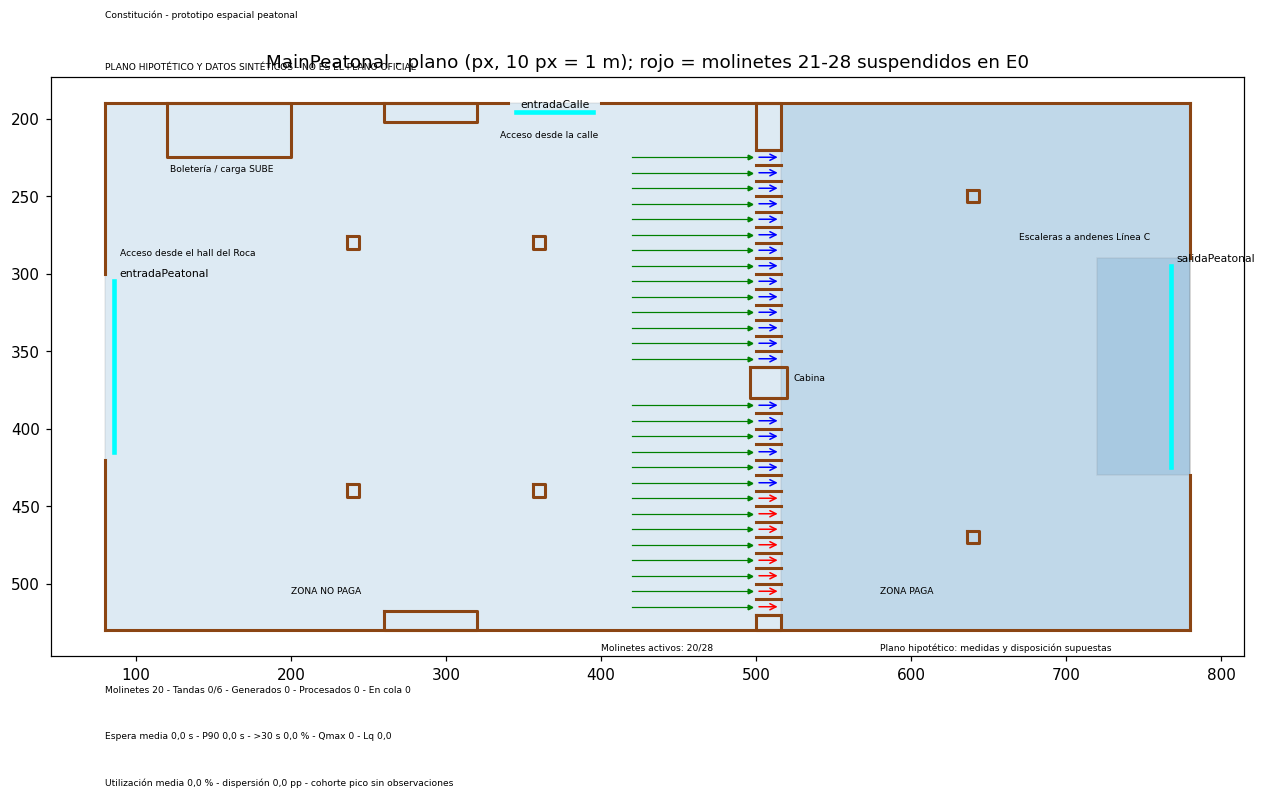
\includegraphics[width=0.9\textwidth]{tpi-subte-plano-hipotetico.png}
\caption{Vestíbulo hipotético: acceso desde el Roca a la izquierda, batería de 28 molinetes en dos bancos
y escaleras a la Línea~C a la derecha. En rojo, los molinetes suspendidos en \EO{}.}
\label{fig:plano}
\end{figure}

\subsection{Lógica de la capa peatonal}

\textbf{Demanda.} Los arribos de los trenes están cargados en el modelo como un arreglo de 61 instantes
entre las 06:30 y las 09:30. Se incluyen los trenes de 06:30 a 07:00 porque, con la demora, su pasaje
llega al vestíbulo después de las 07:00. El perfil de SBASE de la tabla~\ref{tab:perfil} fija el volumen
por ventana. La demanda se genera como se describió en la sección~\ref{sec:paso2-datos-modelo-conceptual}:
\begin{itemize}
  \item el pasaje de cada tren ingresa de forma pareja durante la dispersión de la descarga;
  \item la demanda de la calle se genera por adelgazamiento (\emph{thinning}) de un proceso de Poisson.
\end{itemize}
Si alguno de los cuatro parámetros sin dato no tiene valor, la inicialización se detiene con un error
explícito en lugar de usar un valor oculto.

\textbf{Elección de cola.} \texttt{PedService} delega la elección en una función propia,
\texttt{elegirColaPed}. Para cada molinete habilitado, la función calcula el desvío lateral a 1,3~m/s más
los pasajeros ya asignados a ese molinete que todavía no empezaron a validar, multiplicados por el tiempo
de validación de referencia. El contador incluye a los que caminan hacia la cola y no solo a los que ya
están en ella. Así se evita el \enquote{efecto manada}: una oleada completa eligiendo la misma cola vacía.

\textbf{Medición.} La espera de cada pasajero empieza en el evento \texttt{onEnterQueue} y termina al
comenzar la validación. Las métricas de la franja se congelan a las 09:30 ($t = 9000$), pero la corrida
continúa hasta que sale el último pasajero ingresado antes de esa hora. Recién entonces el modelo escribe
una fila de 17 campos en el archivo de corridas y termina. Antes de escribirla exige que se cumpla
inyectados $=$ generados $=$ procesados. Si no se cumple, se detiene con un error de conservación.

\textbf{Números aleatorios comunes.} Cada fuente de azar tiene su propio generador, sembrado a partir de la
semilla de la réplica: la calle, el tiempo de validación y la velocidad de marcha. La descarga del Roca es
determinística. Por eso \EO{} y \EI{} con la misma semilla reciben exactamente los mismos pasajeros, en
los mismos instantes y con los mismos tiempos de validación \parencite[cap.~11]{law2015}. Lo único que
cambia entre los dos escenarios de un par es la cantidad de molinetes habilitados.

\textbf{Automatización.} El experimento de variación de parámetros \texttt{PeatonalCorridasApareadas}
ejecuta 60 corridas en secuencia. La corrida $j$ usa la semilla $20260923 + \lfloor j/2 \rfloor$ y 20 o 22
molinetes según $j$ sea par o impar. Cada par consecutivo comparte la semilla. Un script
(\texttt{cargar\_corridas.py}) valida las filas y las transfiere a la planilla de análisis sin
transcripción manual. Rechaza filas de demostración, corridas incompletas, pares sin \EO{} o \EI{}, pares
con distinta demanda y violaciones de conservación.

\subsection{Verificación}

La verificación comprueba que el programa hace lo que el modelo conceptual especifica. Se hizo en tres
niveles.

\textbf{Verificador automático.} El script \texttt{verificar\_modelo.py} revisa el archivo del modelo sin
modificarlo:
\begin{itemize}
  \item la estructura del XML, la unicidad de los identificadores y las referencias entre elementos;
  \item los parámetros de cada experimento;
  \item que el horario cargado en el modelo sea exactamente el extraído de los PDF oficiales;
  \item la orientación de las 28 colas.
\end{itemize}
Además compila las funciones Java del modelo contra las bibliotecas instaladas de AnyLogic. Las ejercita
en un arnés de prueba con casos de resultado conocido:
\begin{itemize}
  \item \EO{} suspende 8 molinetes y \EI{}, 6;
  \item una oleada se reparte entre colas en lugar de amontonarse en una;
  \item quien encuentra el molinete libre tiene espera cero y no se le suma la caminata;
  \item no se generan ingresos a partir de las 09:30;
  \item la proporción de pasajeros que llega en tren y la que llega desde la calle coinciden con las
        configuradas;
  \item \EO{} y \EI{} reciben los mismos ingresos y sortean los mismos tiempos de validación;
  \item la media empírica del servicio triangular coincide con la teórica;
  \item la fila de salida tiene los 17 campos en el orden de la planilla.
\end{itemize}
También comprueba que la planilla calcula los mismos intervalos de confianza que una implementación
independiente en Python, con una diferencia menor que $10^{-6}$. La última ejecución, del 27/10/2026,
pasó todos los controles.

\textbf{Traza manual.} En la capa lógica se reprodujo una oleada de 5 pasajeros con 2 molinetes y 3~s de
servicio, cuyo resultado se calcula a mano. Las esperas son 0, 0, 3, 3 y 6~s: espera media de 2,4~s, P90
de 6~s, cola máxima de 3, área bajo la cola de 12 pasajero-segundo y ocupación de 15 molinete-segundo. El
modelo da exactamente esos valores.

\textbf{Controles en cada corrida.} Cada réplica de producción comprueba la conservación y que haya
drenado por completo. Si la corrida termina sin vaciar el sistema, emite una fila marcada como
\texttt{INCOMPLETO} que el cargador rechaza.

\subsection{Control de versiones}

El modelo, los scripts, los datos procesados y este informe se guardan en un repositorio Git. Para evitar
que el IDE y un editor externo se pisen, el archivo del modelo tiene un solo editor por vez. Al cerrar el
IDE se revisa la diferencia con la versión anterior, se corre el verificador y se registra el cambio. Las
salidas de cada corrida se versionan junto al modelo que las produjo.
